%% Author_tex.tex
%% V1.1
%% 2012/18/6
%% Revised on 2015/20/1
%%
%% developed by Techset
%%
%% This file describes the coding for ptephy_v1.cls

%\documentclass{ptephy_v1}%%%%where ptephy_v1 is the template name
\documentclass[preprint]{ptephy_v1}%%%%%% to generate preprint number
%\documentclass{ptephy_v1}%%%%%% to generate preprint number with ptep logo

\preprintnumber{XXXX-XXXX} %%% %%% Insert preprint number here

%The authors can define any packages after the \documentclass{ptephy_v1} command.

%\usepackage[T1]{CJKutf8}
\usepackage[whole]{bxcjkjatype}

\usepackage{amsmath}
\usepackage{amsthm}
\usepackage{hyperref}
\usepackage{graphics}
%\usepackage{algorithmic} for describing algorithms
%\usepackage{subfig} for getting the subfigures e.g., "Figure 1a and 1b" etc.
\usepackage{url}
\usepackage{tikz}
\usetikzlibrary{positioning,arrows.meta}

%The author can find the documentation of additional supporting files from "http://www.ctan.org"

% *** Do not adjust lengths that control margins, column widths, etc. ***

\newtheorem{theorem}{Theorem}
\newtheorem{condition}{Condition}

\begin{document}
%\begin{CJK}{UTF8}{ipxm}

\title{Joint Research of Optics and Fluid Interface}

%%%% To generate auto affiliation numbers please use \author{}\affil{} command

\author{Doumu/Fudepia}
\affil{\email{fudepia@outlook.jp}}

\begin{abstract}
    The abstract text goes here. The abstract text goes here. The abstract text goes here.
    The abstract text goes here. The abstract text goes here. The abstract text goes here.
    The abstract text goes here. The abstract text goes here. The abstract text goes here.
\end{abstract}


\subjectindex{xxxx, xxx}

\maketitle


\section{Regarding Special Relativity}
So first let the real velocity \(v_\text{リ}\), whom maintains the linear properties of traditional non-relativistic velocity.

\begin{equation}
    v_S=\frac{v_\text{リ}\text{エ}_S\text{リ}}{\text{エ}_SS}
\end{equation}

\section{Model of Particles}

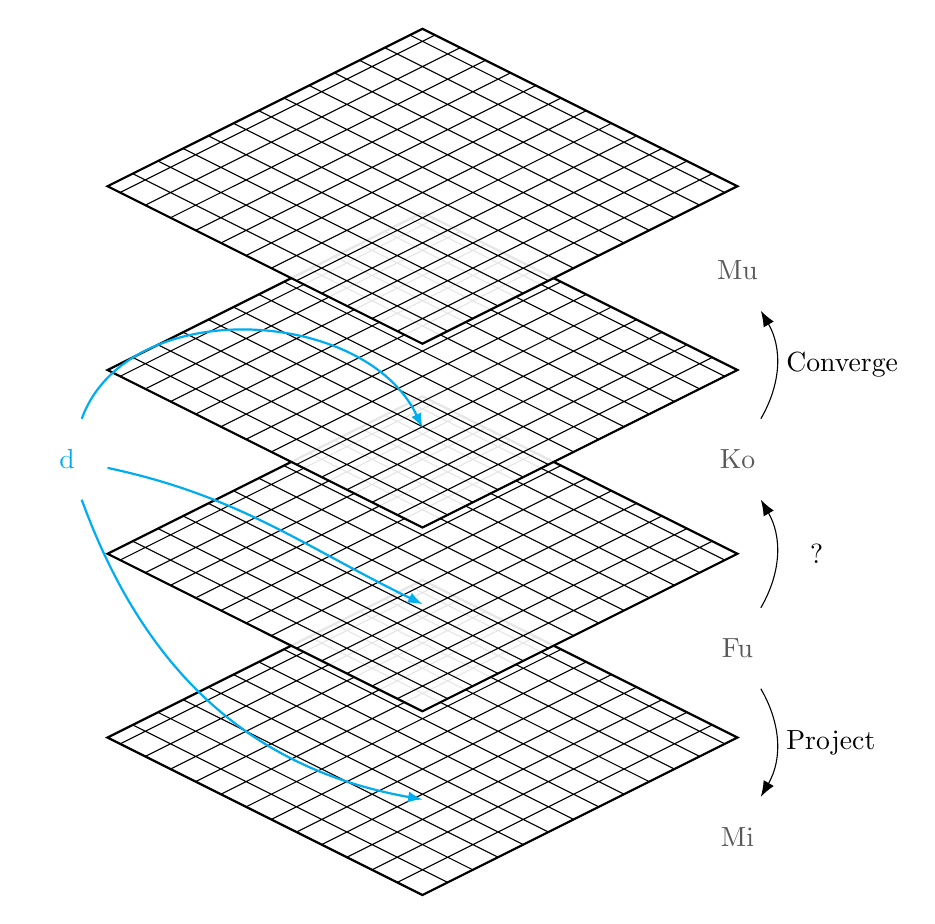
\begin{tikzpicture}[scale=.8,every node/.style={minimum size=1cm},on grid]
    %
    \begin{scope}[
            yshift=-83,every node/.append style={
                yslant=0.5,xslant=-1},yslant=0.5,xslant=-1
        ]
        \draw[step=4mm, black] (0,0) grid (5,5);
        \draw[black,thick] (0,0) rectangle (5,5);%borders
    \end{scope}
    %
    \begin{scope}[
            yshift=0,every node/.append style={
                yslant=0.5,xslant=-1},yslant=0.5,xslant=-1
        ]
        \fill[white,fill opacity=0.9] (0,0) rectangle (5,5);
        \draw[step=4mm, black] (0,0) grid (5,5); %grid definition
        \draw[black,thick] (0,0) rectangle (5,5);%borders
    \end{scope}
    %
    \begin{scope}[
            yshift=83,every node/.append style={
                yslant=0.5,xslant=-1},yslant=0.5,xslant=-1
        ]
        \fill[white,fill opacity=0.9] (0,0) rectangle (5,5);
        \draw[step=4mm, black] (0,0) grid (5,5);
        \draw[black,thick] (0,0) rectangle (5,5);%borders
    \end{scope}
    %
    \begin{scope}[
            yshift=166,every node/.append style={
                yslant=0.5,xslant=-1},yslant=0.5,xslant=-1
        ]
        \fill[white,fill opacity=0.9] (0,0) rectangle (5,5);
        \draw[step=4mm, black] (0,0) grid (5,5);
        \draw[black,thick] (0,0) rectangle (5,5);%borders
    \end{scope}
    %
    \draw[thick,gray!70!black](5,7) node (Mu) {Mu};
    \draw[thick,gray!70!black](5,4) node (Ko) {Ko};
    \draw[thick,gray!70!black](5,1) node (Fu) {Fu};
    \draw[thick,cyan](-5,4) node[left] (Type) {d};
    \draw
    (Type) edge[cyan,thick,-latex,out=70,in=-245] (0,4.5)
    (Type) edge[cyan,thick,-latex,out=-12,in=154] (0,1.7)
    (Type) edge[cyan,thick,-latex,out=-70,in=170] (0,-1.4);
    \draw[thick,gray!70!black](5,-2) node (Mi) {Mi};
    \draw
    (Fu) edge[bend left,-{Latex[length=2mm]}] node [right] {Project} (Mi)
    (Ko) edge[bend right,-{Latex[length=2mm]}] node [right] {Converge} (Mu)
    (Fu) edge[bend right,-{Latex[length=2mm]}] node [right] {?} (Ko);
    %
\end{tikzpicture}





\section{Conclusion}
The conclusion text goes here.

\section*{Acknowledgment}

Insert the Acknowledgment text here.

% can use a bibliography generated by BibTeX as a .bbl file
% BibTeX documentation can be easily obtained at:
% http://www.ctan.org/tex-archive/biblio/bibtex/contrib/doc/

%\bibliographystyle{ptephy}
%\bibliography{sample}
%
% once the .bbl file has been generated then place the text in your article.

%This is added by T. Yoneya (editor-in-chief) on 2020/07/09.

\let\doi\relax

%without this code before the command "\begin{thebibliography}{}" , an error will be %flagged. When the bibliography is provided as separate .bib file, then this code %should be placed above the commands "\bibliographystyle{}" and "\bibliography{}" %inside the main TeX file. 

\begin{thebibliography}{9}

    \bibitem{mucoe}
        \url{https://www.mail-archive.com/dou-geometry@googlegroups.com/msg00004/____________-___________________________.docx}

\end{thebibliography}

\appendix

\section{Appendix head}



%\end{CJK}
\end{document}
